\documentclass{standalone}
\usepackage{tikz}
\usetikzlibrary{patterns, positioning}
\usepackage[sfdefault]{ClearSans} %% option 'sfdefault' activates Clear Sans as the default text font
\usepackage[T1]{fontenc}

\begin{document}
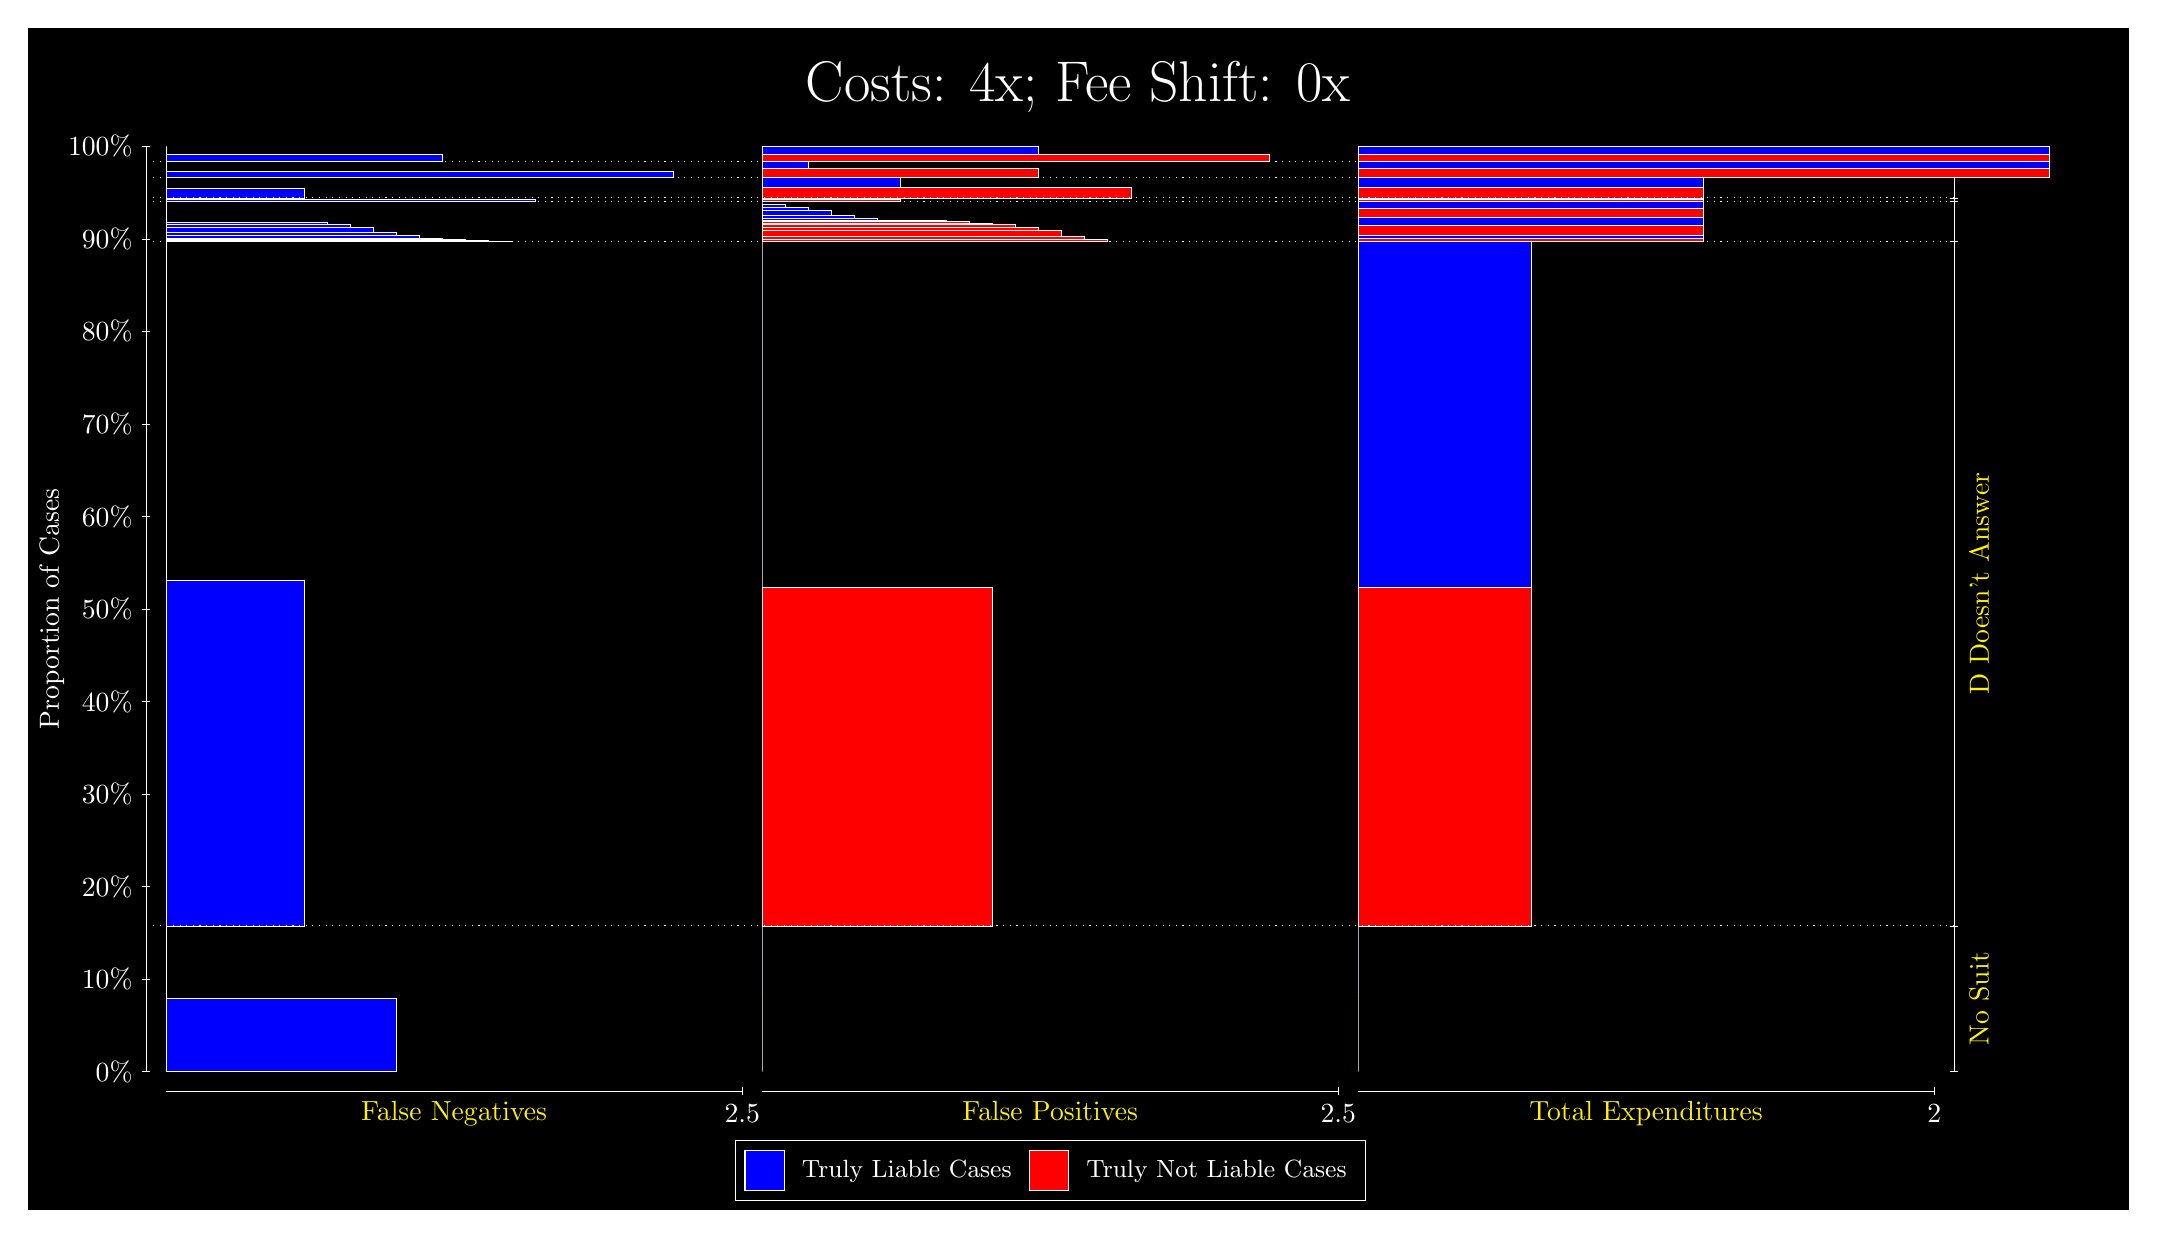
\begin{tikzpicture}
\draw[fill=black] (0,0) rectangle (26.667,15);
\draw[text=white] (0,13.5) rectangle (26.667,15) node[midway] {\huge Costs: 4x; Fee Shift: 0x};
\draw[white, very thin] (1.5,1.75) -- (1.5,13.5);
\node[rotate=90, text=white, anchor=center] at (0.3, 7.625) {Proportion of Cases};
\draw[white, very thin] (1.45,1.75) -- (1.55,1.75);
\node[text=white, anchor=east] at (1.45, 1.75) {0\%};
\draw[white, very thin] (1.45,2.925) -- (1.55,2.925);
\node[text=white, anchor=east] at (1.45, 2.925) {10\%};
\draw[white, very thin] (1.45,4.1) -- (1.55,4.1);
\node[text=white, anchor=east] at (1.45, 4.1) {20\%};
\draw[white, very thin] (1.45,5.275) -- (1.55,5.275);
\node[text=white, anchor=east] at (1.45, 5.275) {30\%};
\draw[white, very thin] (1.45,6.45) -- (1.55,6.45);
\node[text=white, anchor=east] at (1.45, 6.45) {40\%};
\draw[white, very thin] (1.45,7.625) -- (1.55,7.625);
\node[text=white, anchor=east] at (1.45, 7.625) {50\%};
\draw[white, very thin] (1.45,8.8) -- (1.55,8.8);
\node[text=white, anchor=east] at (1.45, 8.8) {60\%};
\draw[white, very thin] (1.45,9.975) -- (1.55,9.975);
\node[text=white, anchor=east] at (1.45, 9.975) {70\%};
\draw[white, very thin] (1.45,11.15) -- (1.55,11.15);
\node[text=white, anchor=east] at (1.45, 11.15) {80\%};
\draw[white, very thin] (1.45,12.325) -- (1.55,12.325);
\node[text=white, anchor=east] at (1.45, 12.325) {90\%};
\draw[white, very thin] (1.45,13.5) -- (1.55,13.5);
\node[text=white, anchor=east] at (1.45, 13.5) {100\%};

\draw[white, very thin] (24.457,1.75) -- (24.457,13.5);
\draw[white, very thin] (24.407,1.75) -- (24.507,1.75);
\node[anchor=west] at (24.407, 1.75) {};
\draw[white, very thin] (24.407,3.5995) -- (24.507,3.5995);
\node[anchor=west] at (24.407, 3.5995) {};
\draw[white, very thin] (24.407,12.292) -- (24.507,12.292);
\node[anchor=west] at (24.407, 12.292) {};
\draw[white, very thin] (24.407,12.804) -- (24.507,12.804);
\node[anchor=west] at (24.407, 12.804) {};
\draw[white, very thin] (24.407,12.846) -- (24.507,12.846);
\node[anchor=west] at (24.407, 12.846) {};
\draw[white, very thin] (24.407,13.104) -- (24.507,13.104);
\node[anchor=west] at (24.407, 13.104) {};
\draw[white, very thin] (24.407,13.304) -- (24.507,13.304);
\node[anchor=west] at (24.407, 13.304) {};
\draw[white, very thin] (24.407,13.5) -- (24.507,13.5);
\node[anchor=west] at (24.407, 13.5) {};

\draw[white, very thin, fill=blue] (1.75,1.75) rectangle (4.6775,2.6748);
\draw[white, very thin, fill=red] (1.75,2.6748) rectangle (1.75,3.5995);
\draw[white, very thin, fill=blue] (1.75,3.5995) rectangle (3.5065,7.9862);
\draw[white, very thin, fill=red] (1.75,7.9862) rectangle (1.75,12.292);
\draw[white, very thin, fill=blue] (1.75,12.292) rectangle (6.1413,12.298);
\draw[white, very thin, fill=blue] (1.75,12.298) rectangle (5.8486,12.308);
\draw[white, very thin, fill=blue] (1.75,12.308) rectangle (5.5558,12.325);
\draw[white, very thin, fill=blue] (1.75,12.325) rectangle (5.2631,12.337);
\draw[white, very thin, fill=blue] (1.75,12.337) rectangle (4.9703,12.376);
\draw[white, very thin, fill=blue] (1.75,12.376) rectangle (4.6775,12.408);
\draw[white, very thin, fill=blue] (1.75,12.408) rectangle (4.3848,12.469);
\draw[white, very thin, fill=blue] (1.75,12.469) rectangle (4.092,12.504);
\draw[white, very thin, fill=blue] (1.75,12.504) rectangle (3.7993,12.53);
\draw[white, very thin, fill=red] (1.75,12.53) rectangle (1.75,12.804);
\draw[white, very thin, fill=blue] (1.75,12.804) rectangle (6.4341,12.823);
\draw[white, very thin, fill=red] (1.75,12.823) rectangle (1.75,12.846);
\draw[white, very thin, fill=blue] (1.75,12.846) rectangle (3.5065,12.966);
\draw[white, very thin, fill=red] (1.75,12.966) rectangle (1.75,13.104);
\draw[white, very thin, fill=blue] (1.75,13.104) rectangle (8.1906,13.189);
\draw[white, very thin, fill=red] (1.75,13.189) rectangle (1.75,13.304);
\draw[white, very thin, fill=blue] (1.75,13.304) rectangle (5.2631,13.404);
\draw[white, very thin, fill=red] (1.75,13.404) rectangle (1.75,13.5);
\draw[white, very thin, fill=red] (9.3189,1.75) rectangle (9.3189,2.6748);
\draw[white, very thin, fill=blue] (9.3189,2.6748) rectangle (9.3189,3.5995);
\draw[white, very thin, fill=red] (9.3189,3.5995) rectangle (12.246,7.9049);
\draw[white, very thin, fill=blue] (9.3189,7.9049) rectangle (9.3189,12.292);
\draw[white, very thin, fill=red] (9.3189,12.292) rectangle (13.71,12.321);
\draw[white, very thin, fill=red] (9.3189,12.321) rectangle (13.417,12.361);
\draw[white, very thin, fill=red] (9.3189,12.361) rectangle (13.125,12.432);
\draw[white, very thin, fill=red] (9.3189,12.432) rectangle (12.832,12.469);
\draw[white, very thin, fill=red] (9.3189,12.469) rectangle (12.539,12.513);
\draw[white, very thin, fill=red] (9.3189,12.513) rectangle (12.246,12.528);
\draw[white, very thin, fill=red] (9.3189,12.528) rectangle (11.954,12.547);
\draw[white, very thin, fill=red] (9.3189,12.547) rectangle (11.661,12.559);
\draw[white, very thin, fill=red] (9.3189,12.559) rectangle (11.368,12.566);
\draw[white, very thin, fill=blue] (9.3189,12.566) rectangle (10.783,12.592);
\draw[white, very thin, fill=blue] (9.3189,12.592) rectangle (10.49,12.627);
\draw[white, very thin, fill=blue] (9.3189,12.627) rectangle (10.197,12.687);
\draw[white, very thin, fill=blue] (9.3189,12.687) rectangle (9.9044,12.72);
\draw[white, very thin, fill=blue] (9.3189,12.72) rectangle (9.6116,12.758);
\draw[white, very thin, fill=blue] (9.3189,12.758) rectangle (9.3189,12.804);
\draw[white, very thin, fill=red] (9.3189,12.804) rectangle (11.075,12.826);
\draw[white, very thin, fill=blue] (9.3189,12.826) rectangle (9.3189,12.846);
\draw[white, very thin, fill=red] (9.3189,12.846) rectangle (14.003,12.983);
\draw[white, very thin, fill=blue] (9.3189,12.983) rectangle (11.075,13.104);
\draw[white, very thin, fill=red] (9.3189,13.104) rectangle (12.832,13.218);
\draw[white, very thin, fill=blue] (9.3189,13.218) rectangle (9.9044,13.304);
\draw[white, very thin, fill=red] (9.3189,13.304) rectangle (15.759,13.4);
\draw[white, very thin, fill=blue] (9.3189,13.4) rectangle (12.832,13.5);
\draw[white, very thin, fill=red] (16.888,1.75) rectangle (16.888,2.6748);
\draw[white, very thin, fill=blue] (16.888,2.6748) rectangle (16.888,3.5995);
\draw[white, very thin, fill=red] (16.888,3.5995) rectangle (19.083,7.9049);
\draw[white, very thin, fill=blue] (16.888,7.9049) rectangle (19.083,12.292);
\draw[white, very thin, fill=red] (16.888,12.292) rectangle (21.279,12.336);
\draw[white, very thin, fill=blue] (16.888,12.336) rectangle (21.279,12.375);
\draw[white, very thin, fill=red] (16.888,12.375) rectangle (21.279,12.493);
\draw[white, very thin, fill=blue] (16.888,12.493) rectangle (21.279,12.597);
\draw[white, very thin, fill=red] (16.888,12.597) rectangle (21.279,12.709);
\draw[white, very thin, fill=blue] (16.888,12.709) rectangle (21.279,12.804);
\draw[white, very thin, fill=red] (16.888,12.804) rectangle (21.279,12.826);
\draw[white, very thin, fill=blue] (16.888,12.826) rectangle (21.279,12.846);
\draw[white, very thin, fill=red] (16.888,12.846) rectangle (21.279,12.983);
\draw[white, very thin, fill=blue] (16.888,12.983) rectangle (21.279,13.104);
\draw[white, very thin, fill=red] (16.888,13.104) rectangle (25.67,13.218);
\draw[white, very thin, fill=blue] (16.888,13.218) rectangle (25.67,13.304);
\draw[white, very thin, fill=red] (16.888,13.304) rectangle (25.67,13.4);
\draw[white, very thin, fill=blue] (16.888,13.4) rectangle (25.67,13.5);
\draw[white, dotted] (1.5,3.5995) -- (24.457,3.5995);
\draw[white, dotted] (1.5,12.292) -- (24.457,12.292);
\draw[white, dotted] (1.5,12.804) -- (24.457,12.804);
\draw[white, dotted] (1.5,12.846) -- (24.457,12.846);
\draw[white, dotted] (1.5,13.104) -- (24.457,13.104);
\draw[white, dotted] (1.5,13.304) -- (24.457,13.304);
\draw[white, very thin] (1.75,1.5) -- (9.0689,1.5);
\node[text=yellow, anchor=north] at (5.4094, 1.5) {False Negatives};
\draw[white, very thin] (9.0689,1.45) -- (9.0689,1.55);
\node[text=white, anchor=north] at (9.0689, 1.45) {2.5};

\draw[white, very thin] (9.3189,1.5) -- (16.638,1.5);
\node[text=yellow, anchor=north] at (12.978, 1.5) {False Positives};
\draw[white, very thin] (16.638,1.45) -- (16.638,1.55);
\node[text=white, anchor=north] at (16.638, 1.45) {2.5};

\draw[white, very thin] (16.888,1.5) -- (24.207,1.5);
\node[text=yellow, anchor=north] at (20.547, 1.5) {Total Expenditures};
\draw[white, very thin] (24.207,1.45) -- (24.207,1.55);
\node[text=white, anchor=north] at (24.207, 1.45) {2};

\node[text=yellow, centered, rotate=90] at (24.777, 2.6748) {No Suit};
\node[text=yellow, centered, rotate=90] at (24.777, 7.9456) {D Doesn't Answer};






\draw (12.978300999999998,1.5) node[draw=none] (baseCoordinate) {};
\begin{scope}[align=center]
        \matrix[scale=0.5, draw=white, below=0.5cm of baseCoordinate, nodes={draw}, column sep=0.1cm]{
            \node[rectangle, draw, minimum width=0.5cm, minimum height=0.5cm, fill=blue] {}; &
            \node[draw=none, font=\small, text=white] (B) {Truly Liable Cases}; &
            \node[rectangle, draw, minimum width=0.5cm, minimum height=0.5cm, fill=red] {}; &
            \node[draw=none, font=\small, text=white] (B) {Truly Not Liable Cases}; \\
            };
\end{scope}

\end{tikzpicture}
\end{document}